\section{Conclusion}
\label{Chap:Al/Vac:section:Conc}


In this chapter, we first demonstrate that the \acf{BEP} relationship fails to provide quantitatively accurate diffusion barriers for multi-component alloys. Then we developed a \ac{NN} model to predict diffusion barriers using thousands of \ac{DFT} calculated barriers. And a \ac{kMC} method based on this \ac{NN} model is used to study the early transition behavior from a supersaturated solid solution to \ac{GP} zone of Al 7000 series alloys. A local super-basin method together with \ac{LRU} cache is also implemented to accelerate \ac{kMC} simulations. Following our general strategy to add a trace amount of element, we studied the effect of adding pseudo-atoms with different ability to change vacancy diffusion barriers. At last, several quantitative analysis to describe the chemical and structural properties of clusters is developed, which could be used as inputs to predict precipitate strengthening effects.


\newpage
\begingroup
\begin{figure}[!ht]
  \centering
  \subfigure[$\varepsilon_{Mg-X} = 0.05$, cluster]{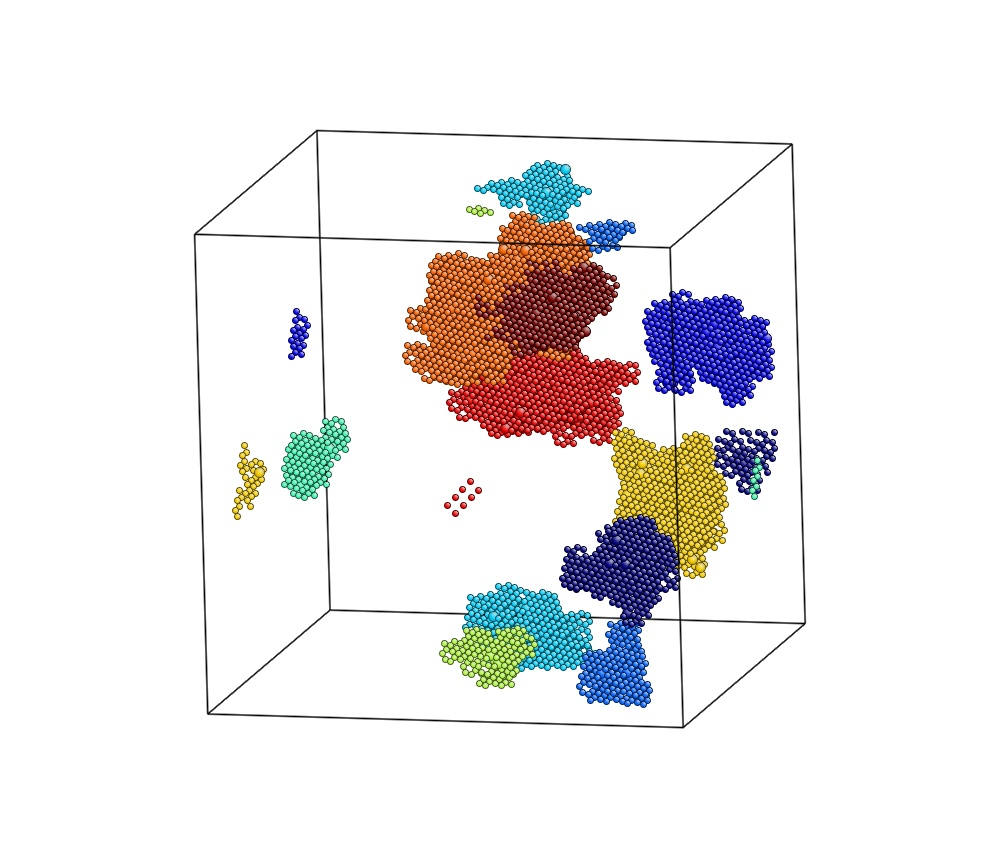
\includegraphics[width=0.49\linewidth]{Chap5/plots/cluster_id_jpg/00003.jpg}}
%   \subfigure[control]{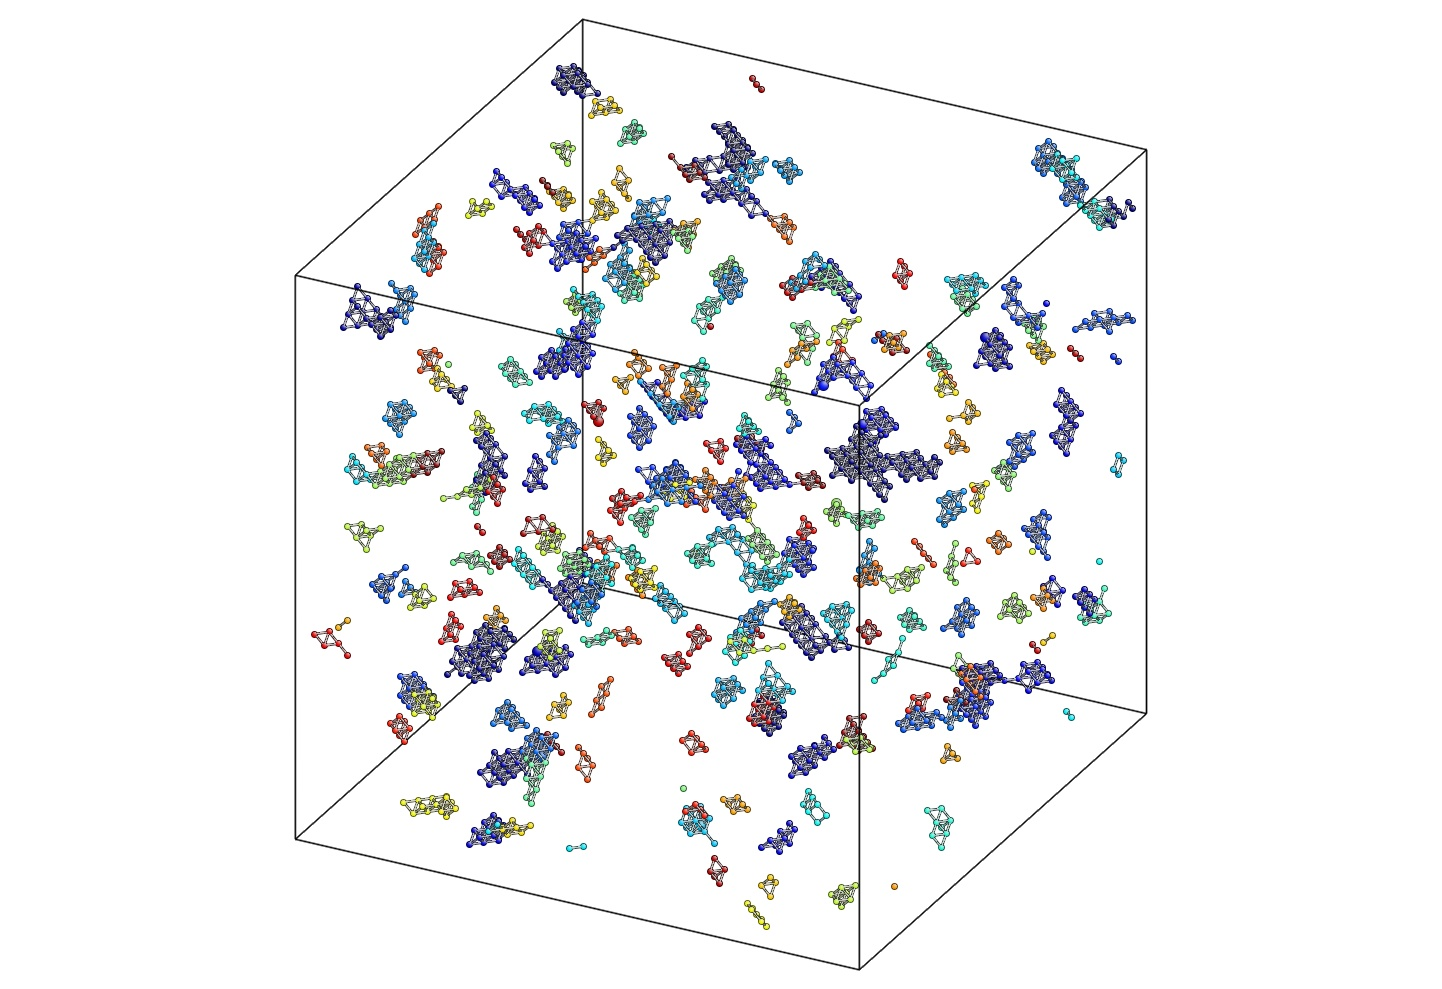
\includegraphics[width=0.32\linewidth]{Chap5/plots/cluster_id_jpg/00000.jpg}}
  \subfigure[$\varepsilon_{Mg-X} = -0.05$, cluster]{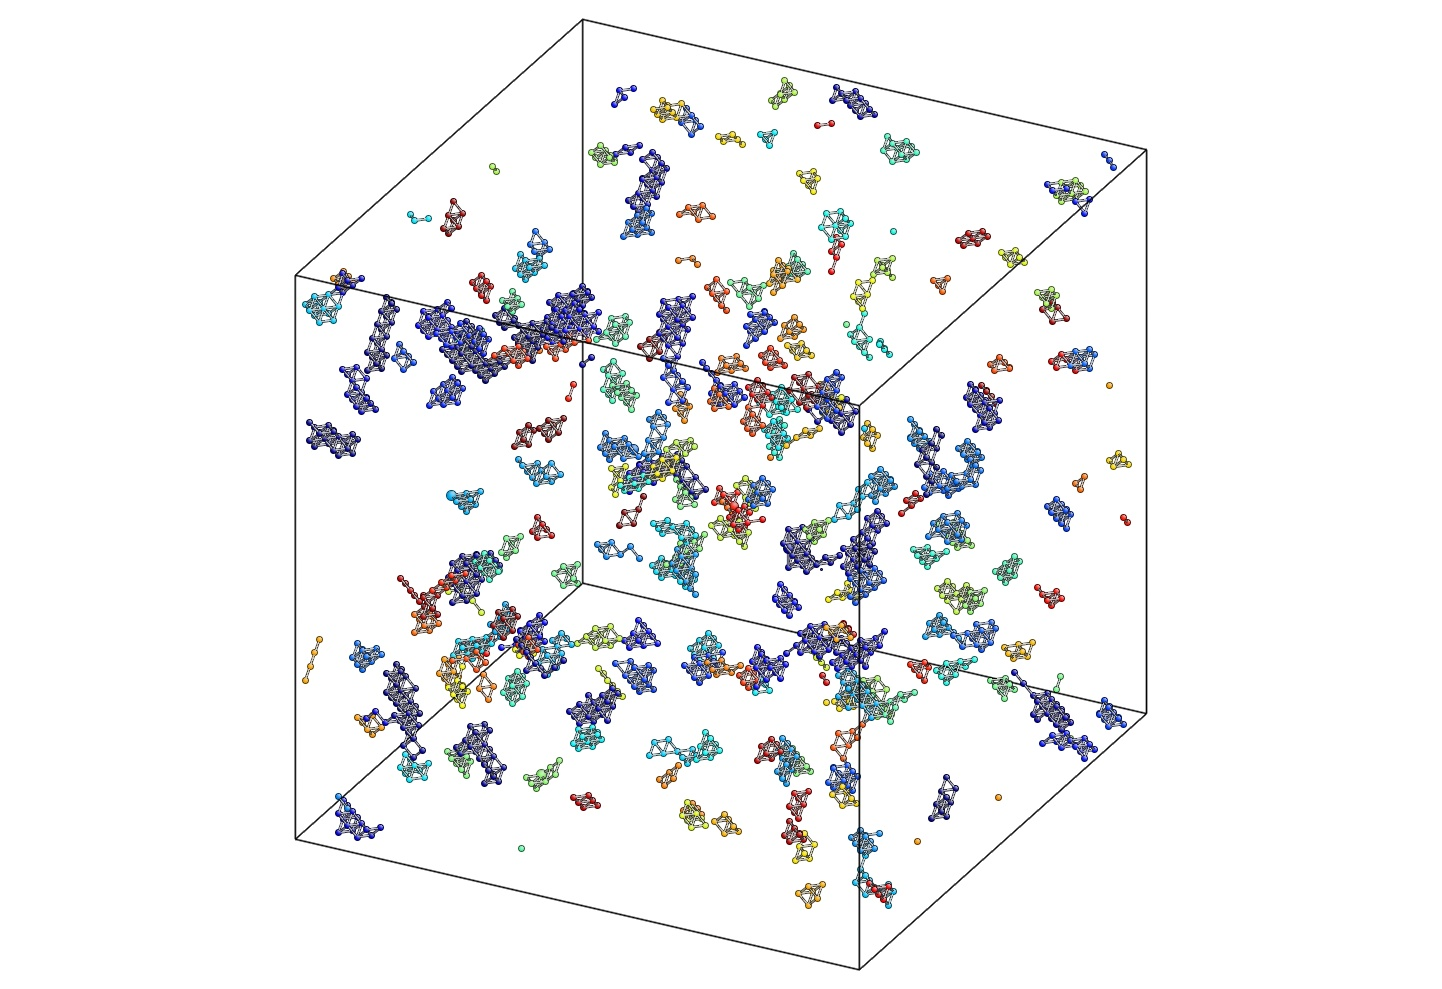
\includegraphics[width=0.49\linewidth]{Chap5/plots/cluster_id_jpg/00004.jpg}} \\
  \subfigure[$\varepsilon_{Mg-X} = 0.05$, species]{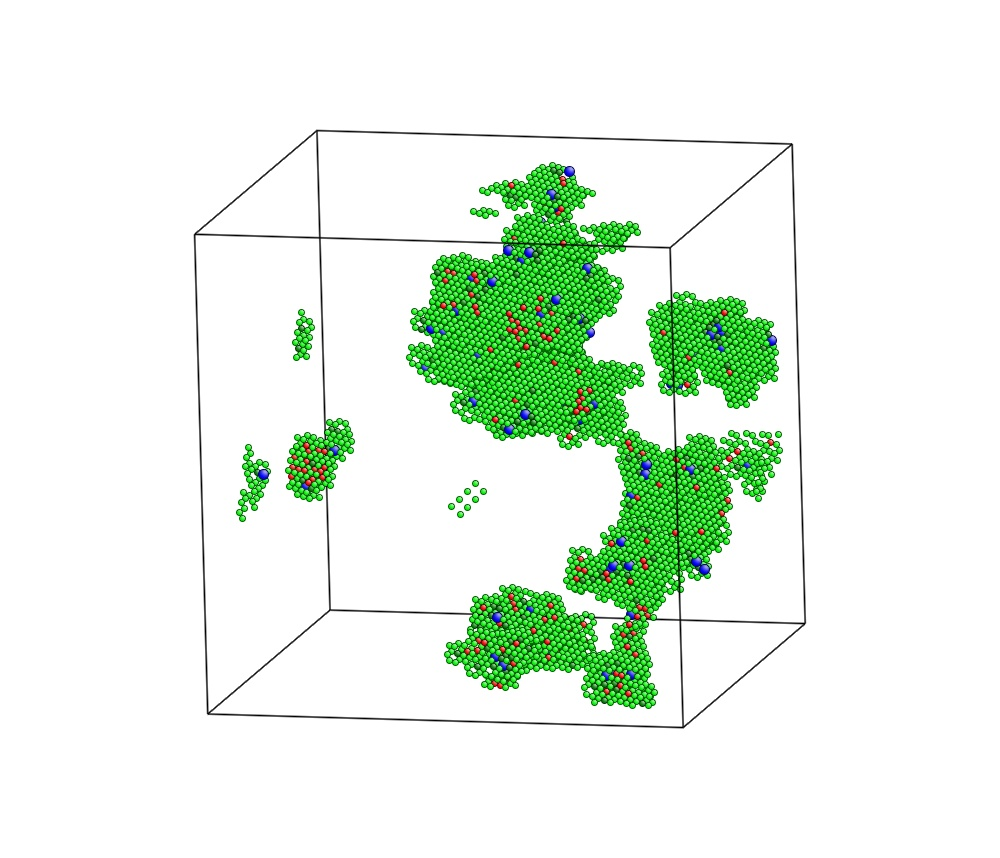
\includegraphics[width=0.49\linewidth]{Chap5/plots/element_jpg/00003.jpg}}
%   \subfigure[control]{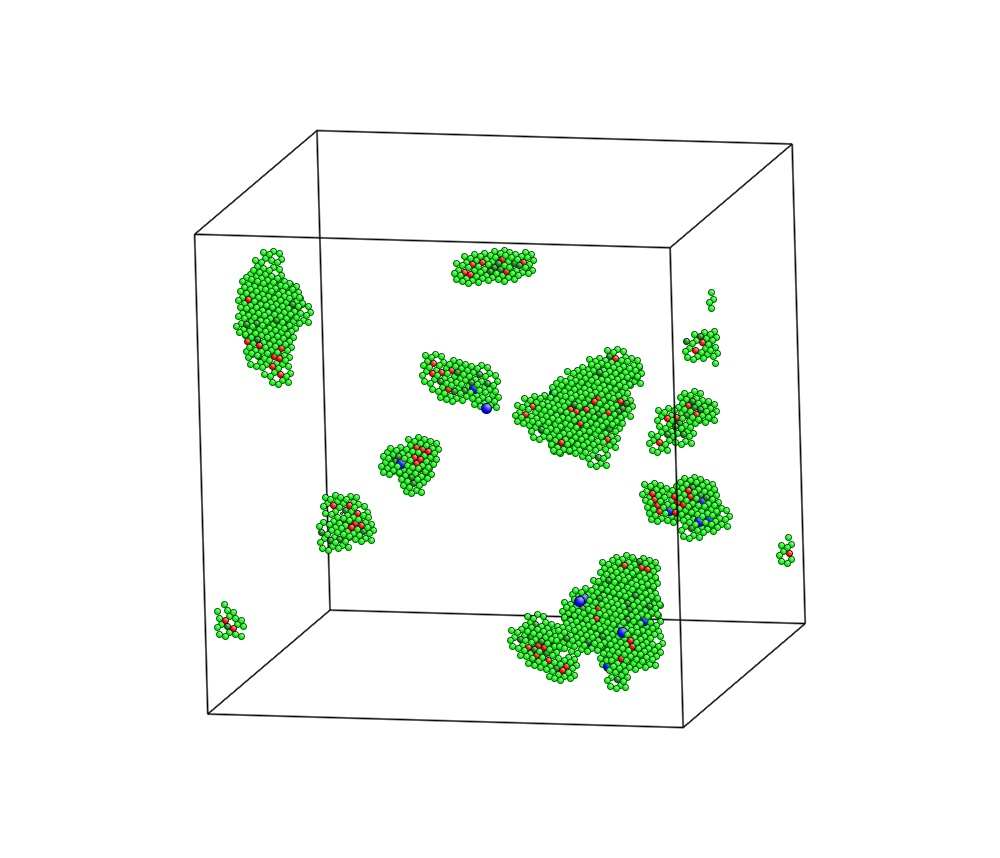
\includegraphics[width=0.32\linewidth]{Chap5/plots/element_jpg/00000.jpg}}
  \subfigure[$\varepsilon_{Mg-X} = -0.05$, species]{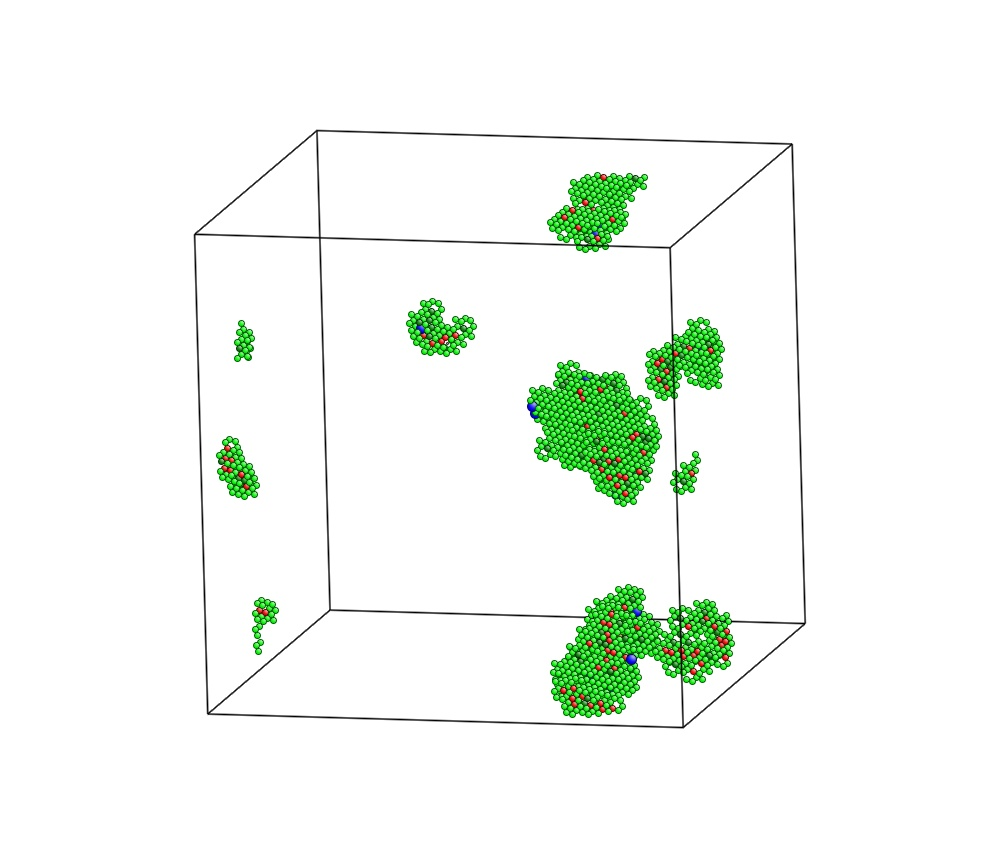
\includegraphics[width=0.49\linewidth]{Chap5/plots/element_jpg/00004.jpg}}
% \caption[Atomistic pictures of 108,000 atoms for $\varepsilon_{Mg-X}$ sensitivity test.]{Atomistic pictures of 108,000 atoms for $\varepsilon_{Mg-X}$ sensitivity test. (a), (d) : $\varepsilon_{Mg-X} = 0.05$, which is setup \#3 in Table. \ref{Chap:Al/Vac:tab:pseudo1}. (b), (e) : setup \#0 in Table. \ref{Chap:Al/Vac:tab:pseudo1}. (c), (f) : $\varepsilon_{Mg-X} = -0.05$, which is setup \#4 in Table. \ref{Chap:Al/Vac:tab:pseudo1}. (a), (b), and (c) are colored by cluster size. The color mapping from dark blue to red is ranked by the cluster size in descending order. (d), (e), and (f) are colored by atom species.  Light green, dark green, red, and blue atoms are Al, Mg, Zn, and pseudo atoms respectively.}
\caption[Atomistic pictures of 108,000 atoms for $\varepsilon_{Mg-X}$ sensitivity test.]{Atomistic pictures of 108,000 atoms for $\varepsilon_{Mg-X}$ sensitivity test. (a), (c) : $\varepsilon_{Mg-X} = 0.05$, which is setup \#3 in Table. \ref{Chap:Al/Vac:tab:pseudo1}. (b), (d) : $\varepsilon_{Mg-X} = -0.05$, which is setup \#4 in Table. \ref{Chap:Al/Vac:tab:pseudo1}. (a) and (c) are colored by cluster size. The color mapping from dark blue to red is ranked by the cluster size in descending order. (b) and (d) are colored by atom species. Light green, dark green, red, and blue atoms are Al, Mg, Zn, and pseudo atoms respectively. And small gray sticks are bonds between atoms.}
\label{Chap:Al/Vac:fig:sens_Mg}
\end{figure}
\endgroup

\newpage
\begingroup
\begin{figure}[!ht]
  \centering
  \subfigure[$\varepsilon_{Zn-X} = 0.05$, cluster]{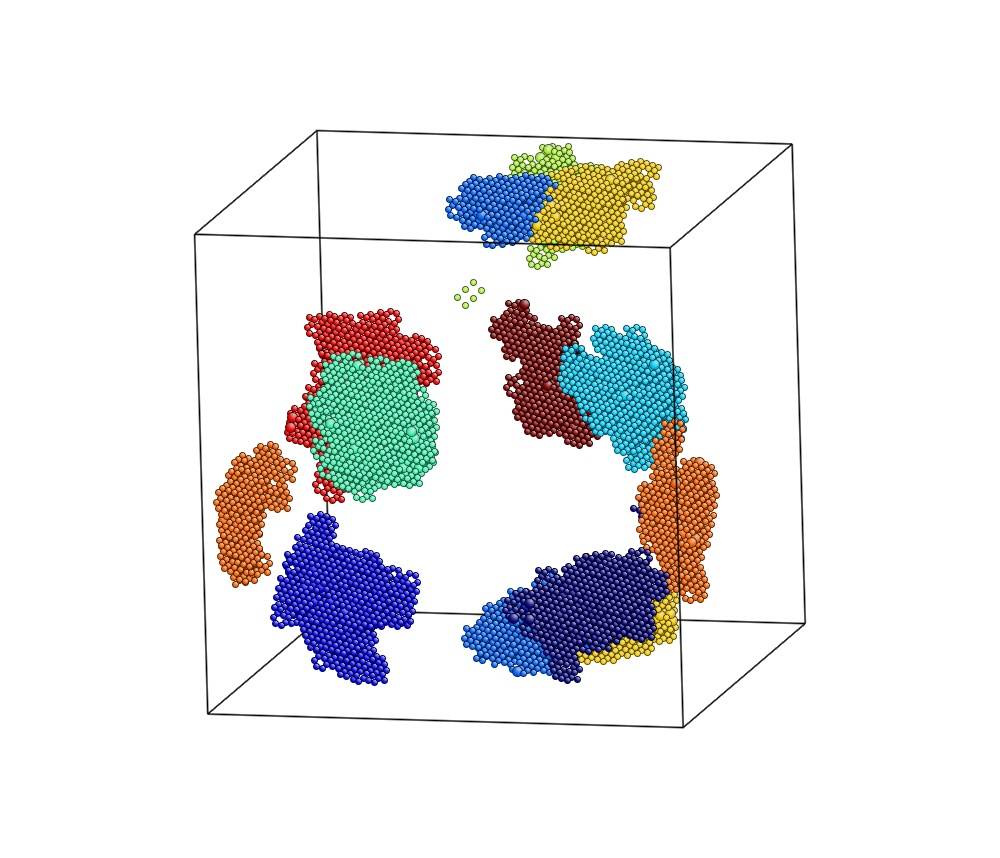
\includegraphics[width=0.49\linewidth]{Chap5/plots/cluster_id_jpg/00005.jpg}}
%   \subfigure[control]{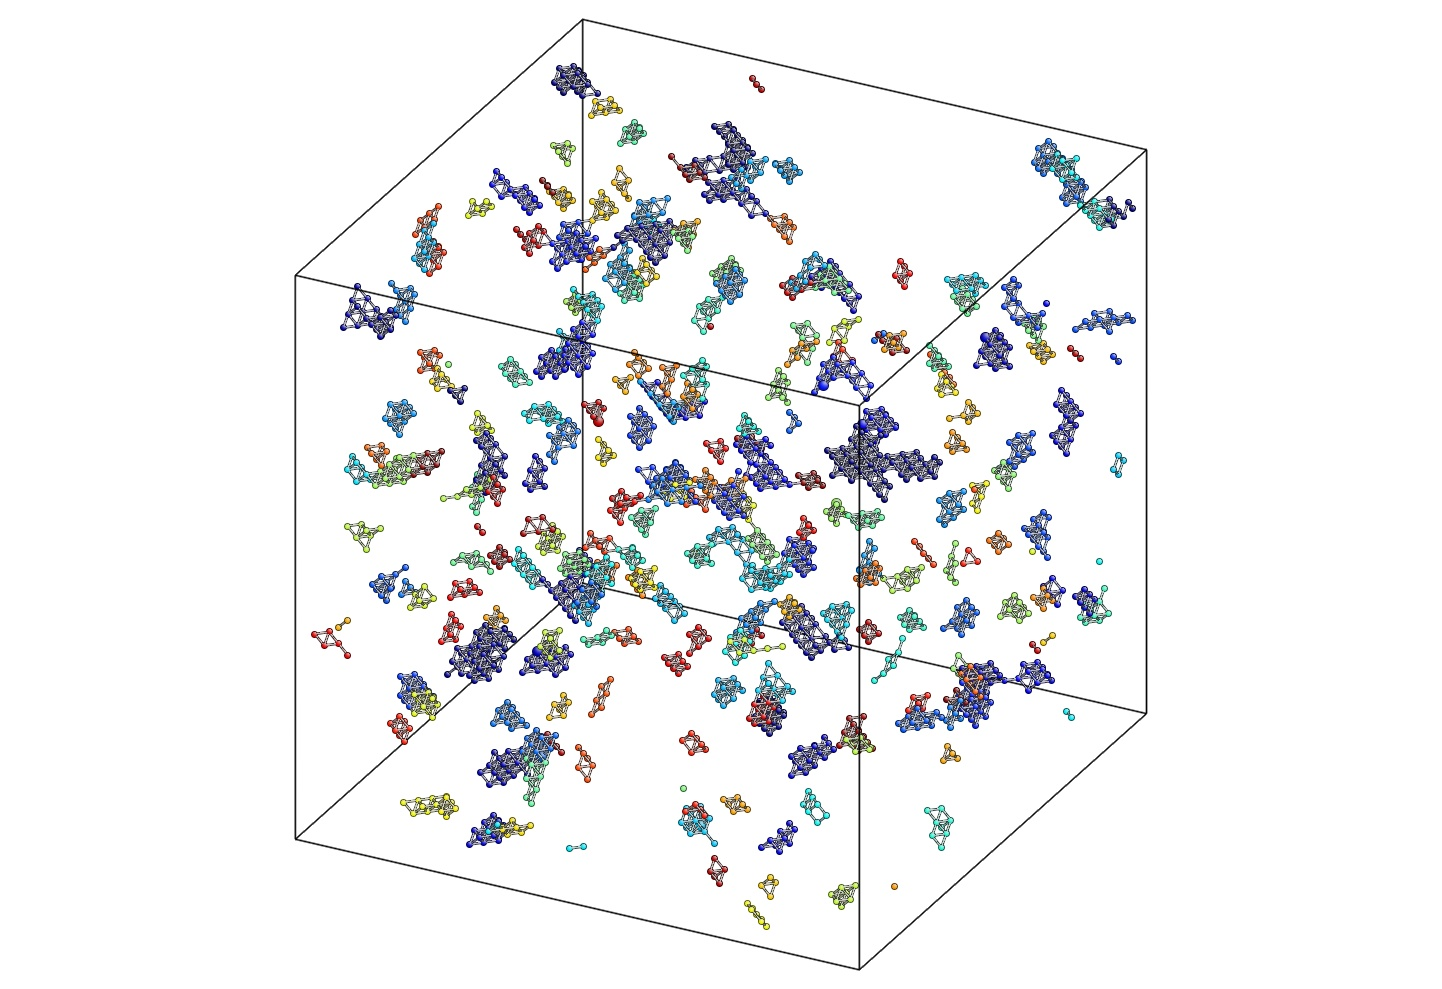
\includegraphics[width=0.32\linewidth]{Chap5/plots/cluster_id_jpg/00000.jpg}}
  \subfigure[$\varepsilon_{Zn-X} = -0.05$, cluster]{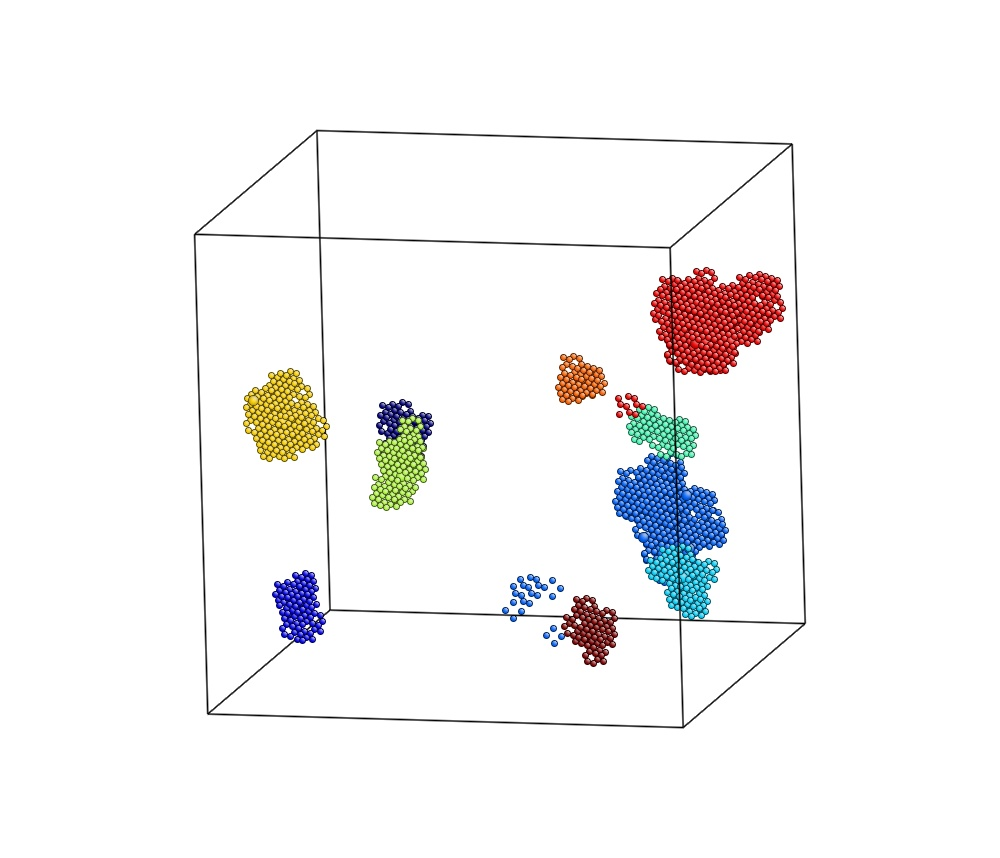
\includegraphics[width=0.49\linewidth]{Chap5/plots/cluster_id_jpg/00006.jpg}} \\
  \subfigure[$\varepsilon_{Zn-X} = 0.05$, species]{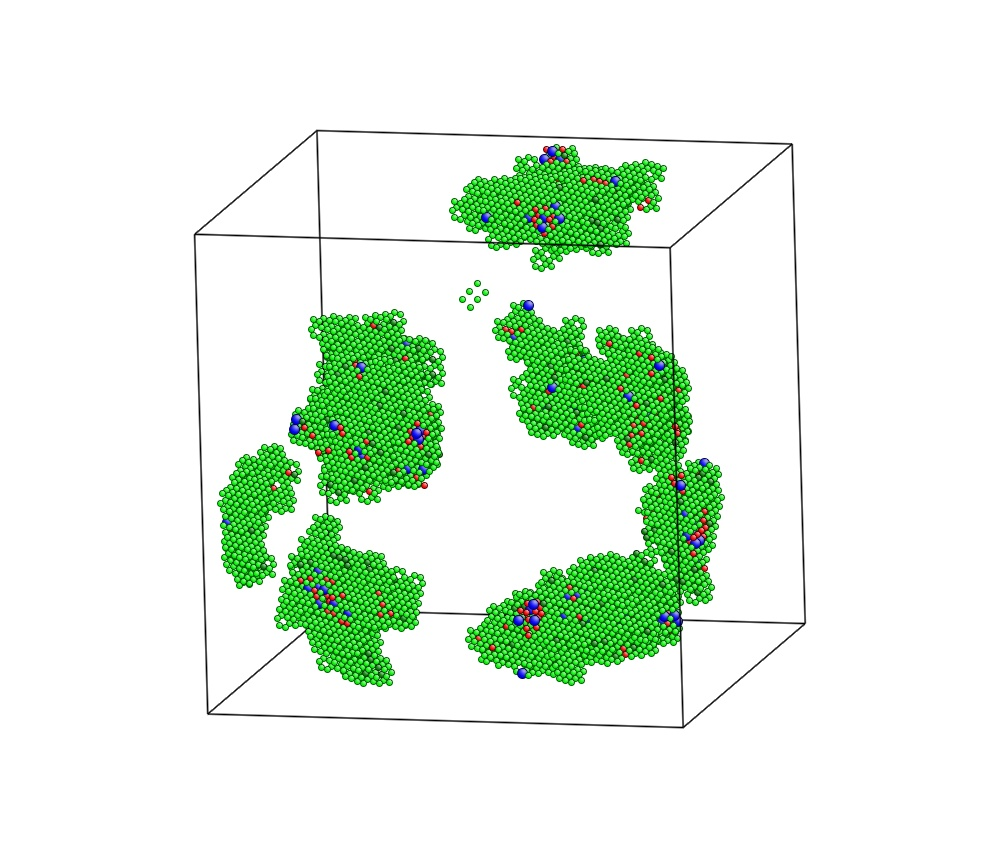
\includegraphics[width=0.49\linewidth]{Chap5/plots/element_jpg/00005.jpg}}
%   \subfigure[control]{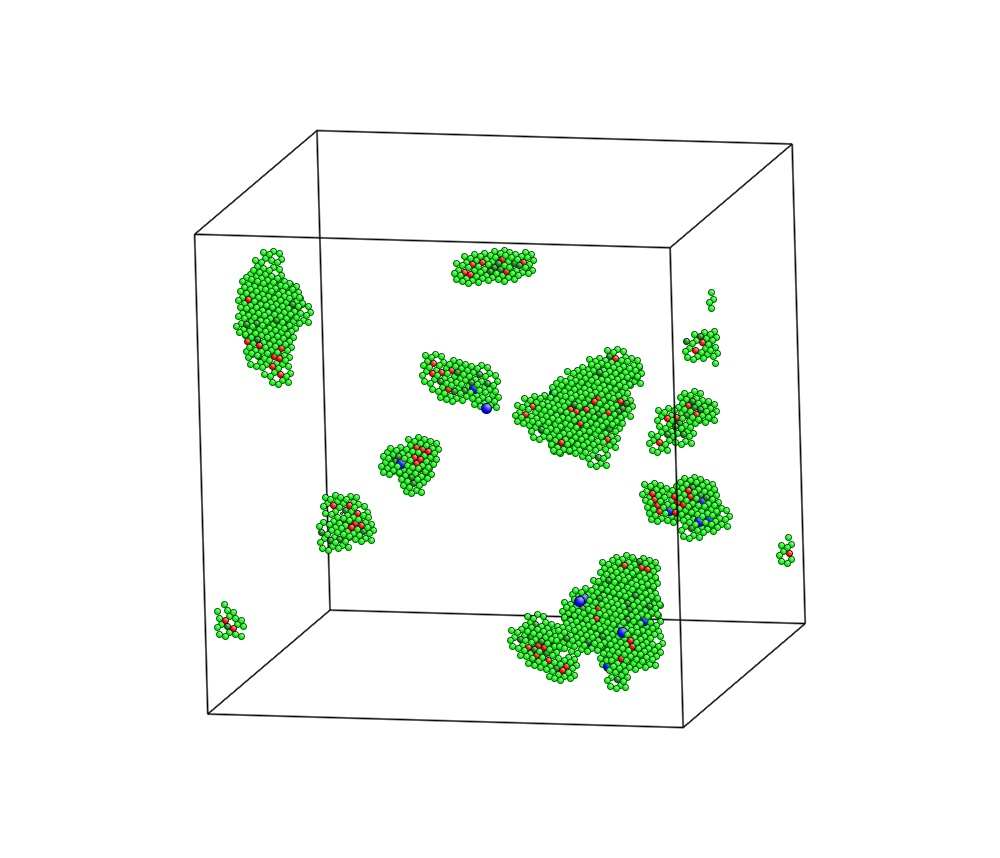
\includegraphics[width=0.32\linewidth]{Chap5/plots/element_jpg/00000.jpg}}
  \subfigure[$\varepsilon_{Zn-X} = -0.05$, species]{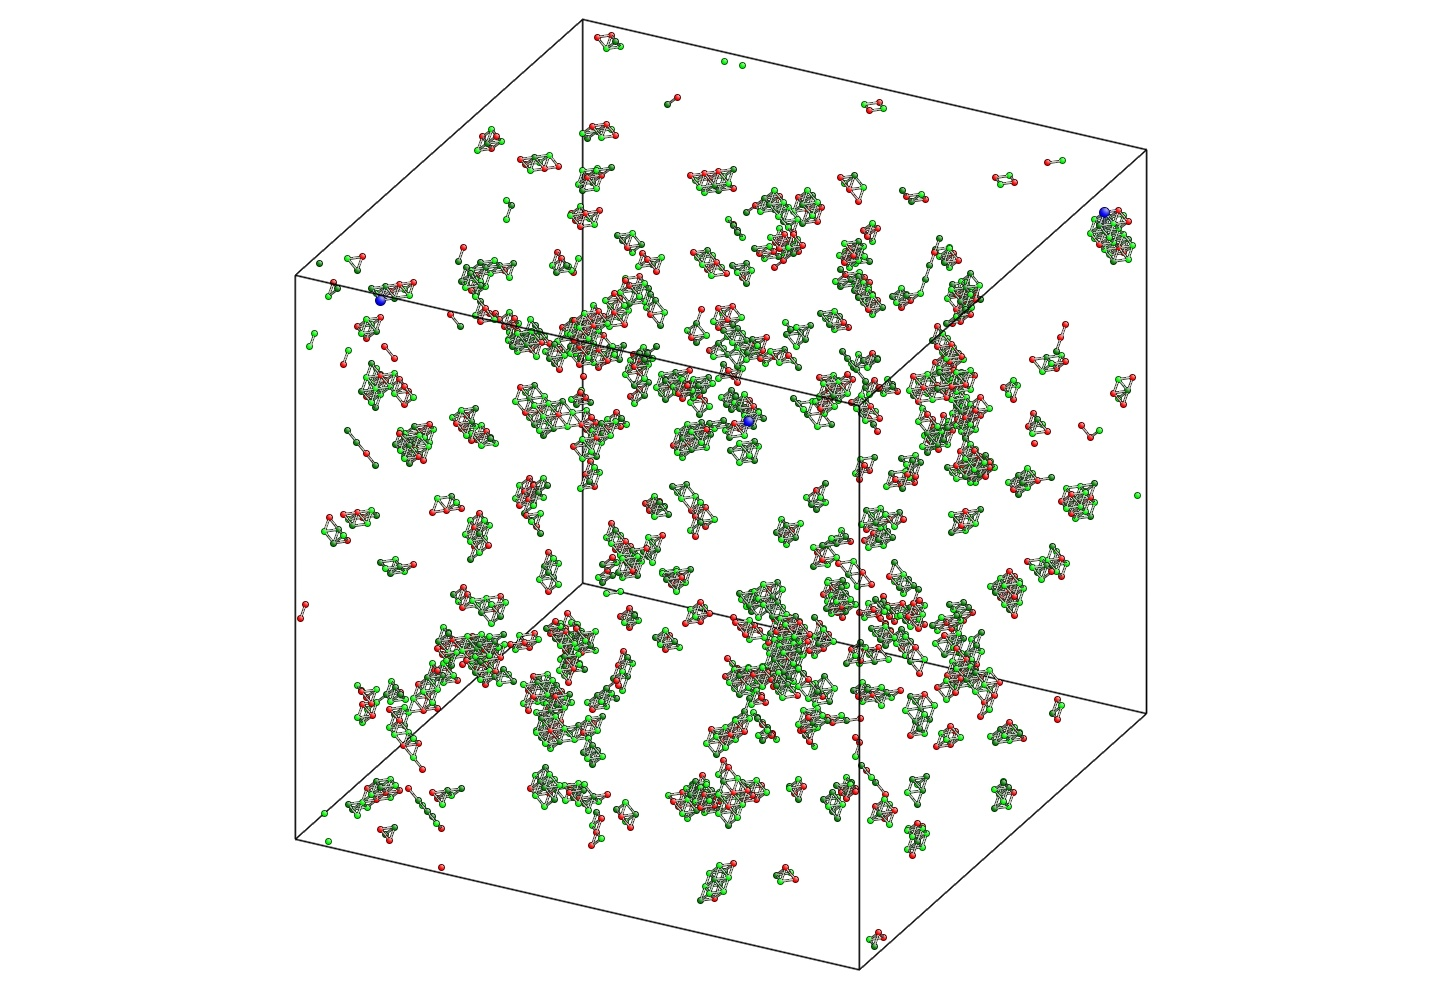
\includegraphics[width=0.49\linewidth]{Chap5/plots/element_jpg/00006.jpg}}
% \caption[Atomistic pictures of 108,000 atoms for $\varepsilon_{Zn-X}$ sensitivity test.]{Atomistic pictures of 108,000 atoms for $\varepsilon_{Zn-X}$ sensitivity test. (a), (d) : $\varepsilon_{Zn-X} = 0.05$, which is setup \#5 in Table. \ref{Chap:Al/Vac:tab:pseudo1}. (b), (e) : setup \#0 in Table. \ref{Chap:Al/Vac:tab:pseudo1}. (c), (f) : $\varepsilon_{Zn-X} = -0.05$, which is setup \#6 in Table. \ref{Chap:Al/Vac:tab:pseudo1}. (a), (b), and (c) are colored by cluster size. The color mapping from dark blue to red is ranked by the cluster size in descending order. (d), (e), and (f) are colored by atom species.  Light green, dark green, red, and blue atoms are Al, Mg, Zn, and pseudo atoms respectively.}
\caption[Atomistic pictures of 108,000 atoms for $\varepsilon_{Zn-X}$ sensitivity test.]{Atomistic pictures of 108,000 atoms for $\varepsilon_{Zn-X}$ sensitivity test. (a), (c) : $\varepsilon_{Zn-X} = 0.05$, which is setup \#5 in Table. \ref{Chap:Al/Vac:tab:pseudo1}. (b), (d) : $\varepsilon_{Zn-X} = -0.05$, which is setup \#6 in Table. \ref{Chap:Al/Vac:tab:pseudo1}. (a) and (c) are colored by cluster size. The color mapping from dark blue to red is ranked by the cluster size in descending order. (b) and (d) are colored by atom species. Light green, dark green, red, and blue atoms are Al, Mg, Zn, and pseudo atoms respectively. And small gray sticks are bonds between atoms.}
\label{Chap:Al/Vac:fig:sens_Zn}
\end{figure}
\endgroup